\documentclass{article}
\usepackage[utf8]{inputenc}
\usepackage{graphicx}
\title{Cara Pembuatan Aplikasi di Oracle APEX}
\author{Almi Bachri (1184043) }
\date{Oktober 2019}

\begin{document}

\maketitle
\begin{enumerate}
    \item Login ke oracle APEX
    \begin{figure}[!htbp]
        \centering
        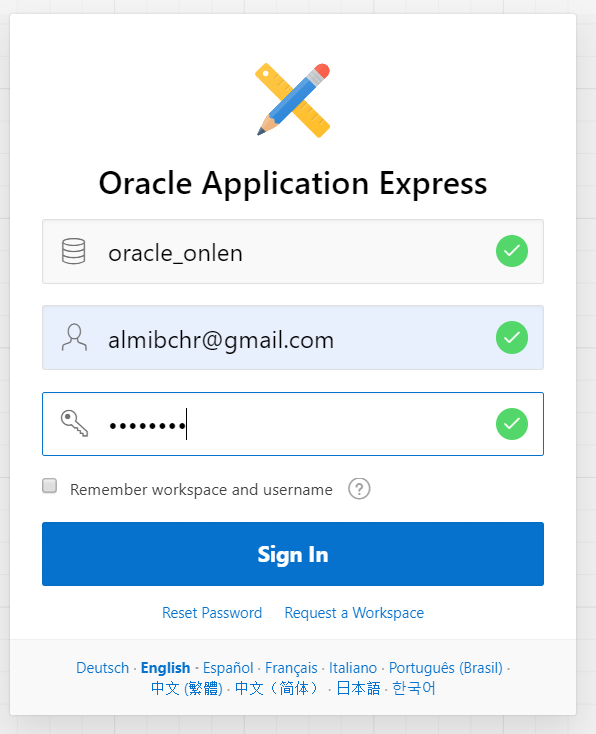
\includegraphics [width=3cm]{figure/Capture.PNG}
        \caption{Caption}
        \label{fig:my_label}
    \end{figure}
    
    \item Pilih "App Builder" lalu klik "Create"
     \begin{figure}[!htbp]
        \centering
        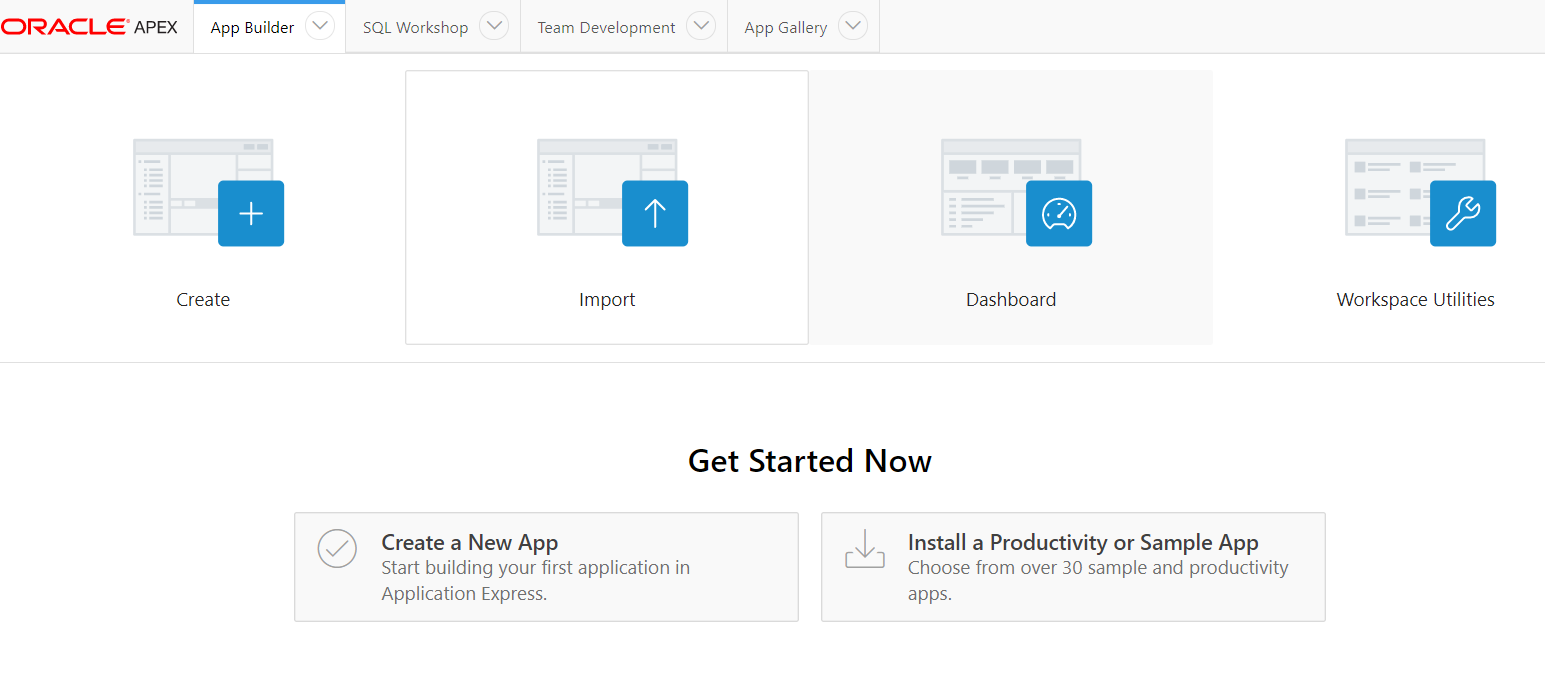
\includegraphics [width=3cm]{figure/Capture1.PNG}
        \caption{Caption}
        \label{fig:my_label}
    \end{figure}
    
    \item Klik "From a File"
     \begin{figure}[!htbp]
        \centering
        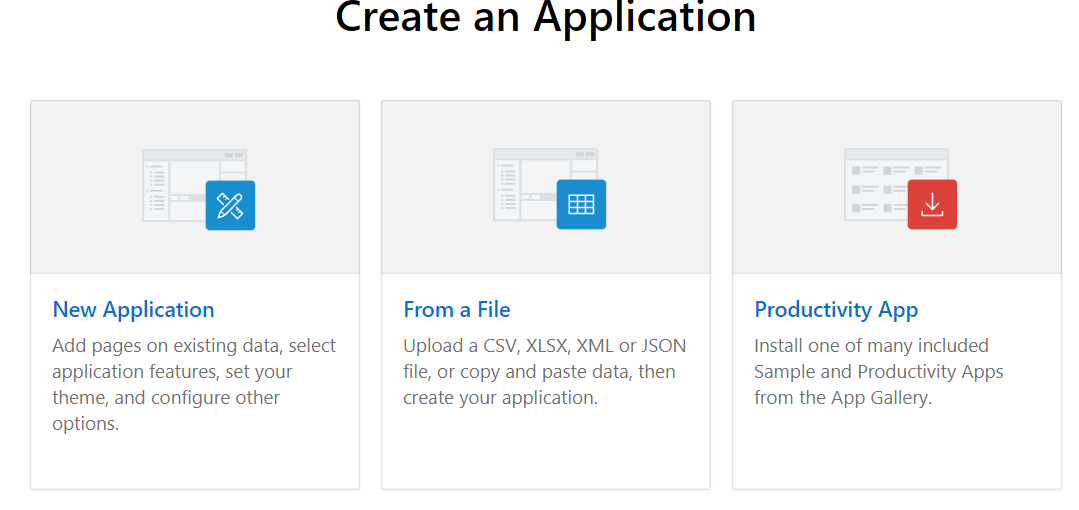
\includegraphics [width=5cm]{figure/Capture2.PNG}
        \caption{Caption}
        \label{fig:my_label}
    \end{figure}
    
    \item Masukkan file yang akan kalian buat, bisa "upload file" atau "copy and paste", kalau saya disini dengan cara "copy and paste" file yang akan dibuat.
     \begin{figure}[!htbp]
        \centering
        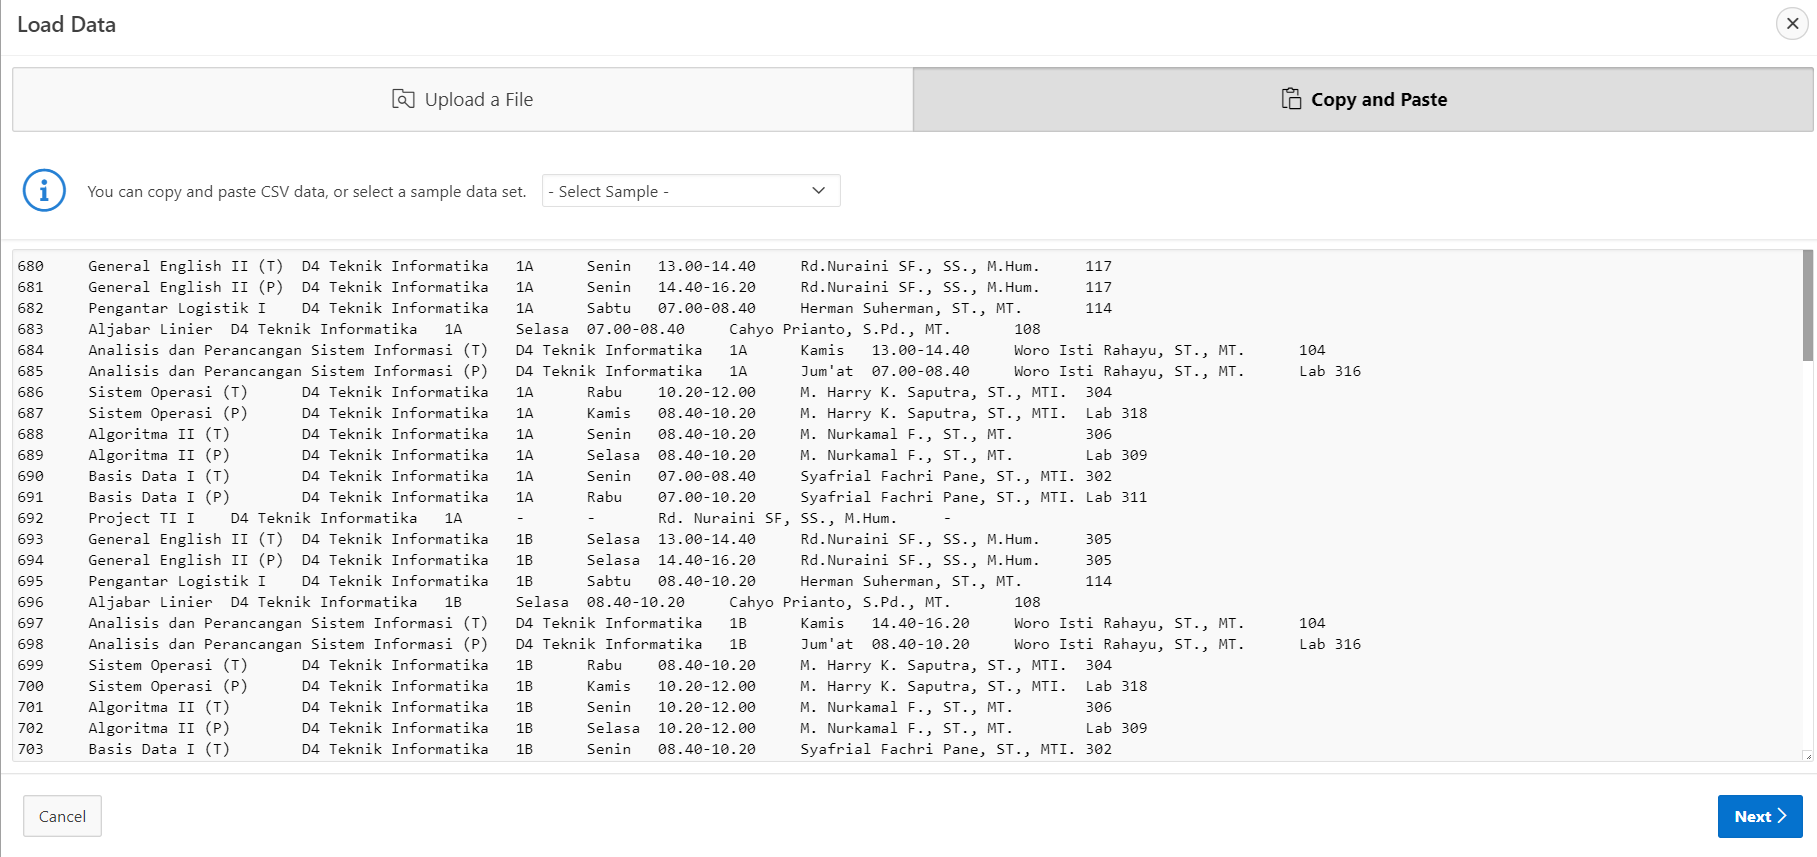
\includegraphics [width=3cm]{figure/Capture3.PNG}
        \caption{Caption}
        \label{capture3}
    \end{figure}
    
    \item Isi "table name" yang akan kalian buat, setelah terisi maka "table name error" akan otomatis terisi, lalu klik "load data"
     \begin{figure}[!htbp]
        \centering
        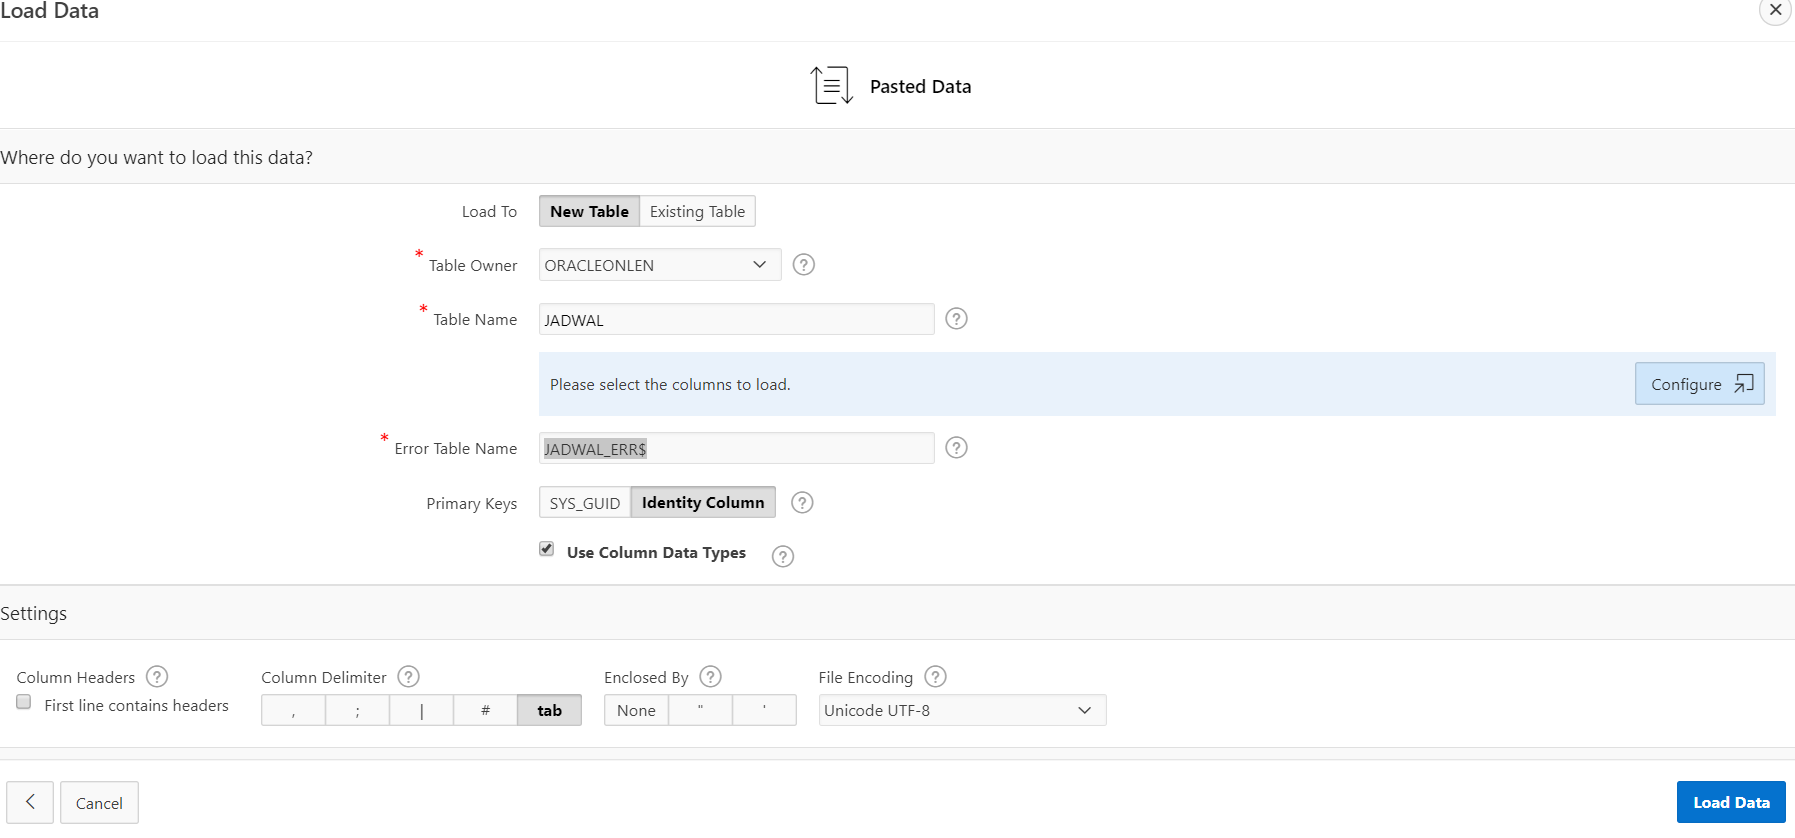
\includegraphics [width=5cm]{figure/Capture4.PNG}
        \caption{Caption}
        \label{fig:my_label}
    \end{figure}
    
    \item Setelah klik "Load Data", maka jika berhasil akan ada ceklis hijau lalu klik View Table
     \begin{figure}[!htbp]
        \centering
        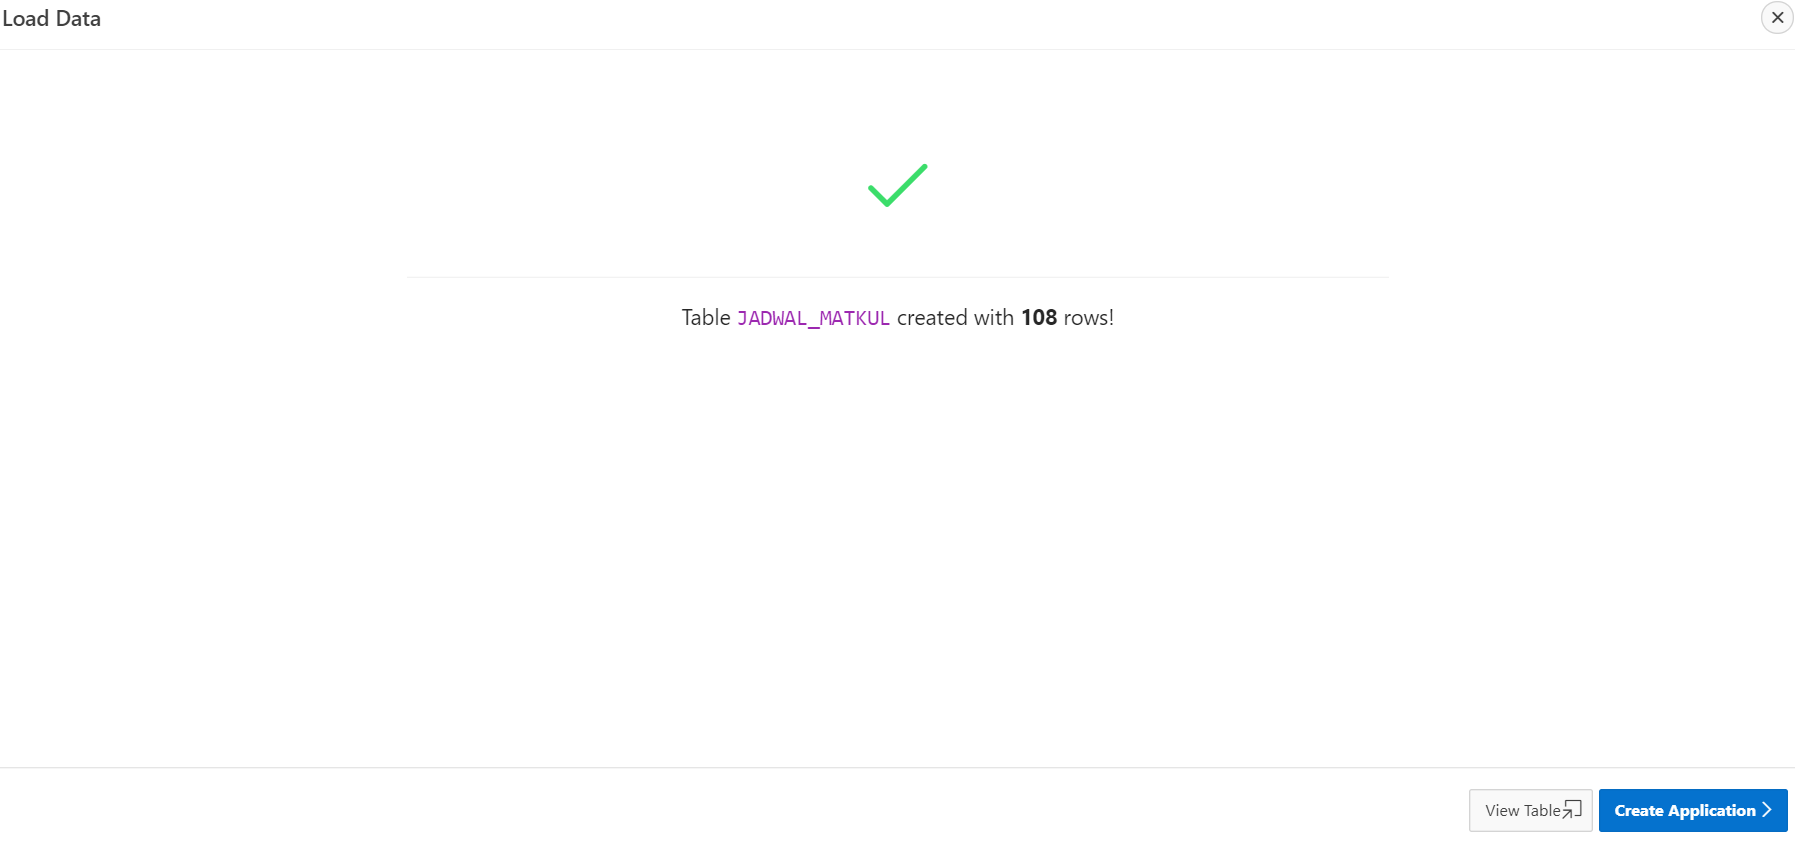
\includegraphics [width=5cm]{figure/Capture5.PNG}
        \caption{Caption}
        \label{fig:my_label}
    \end{figure}
    
    \item Setelah itu, Rename Column namai sesuai tabel yang kalian buat
     \begin{figure}[!htbp]
        \centering
        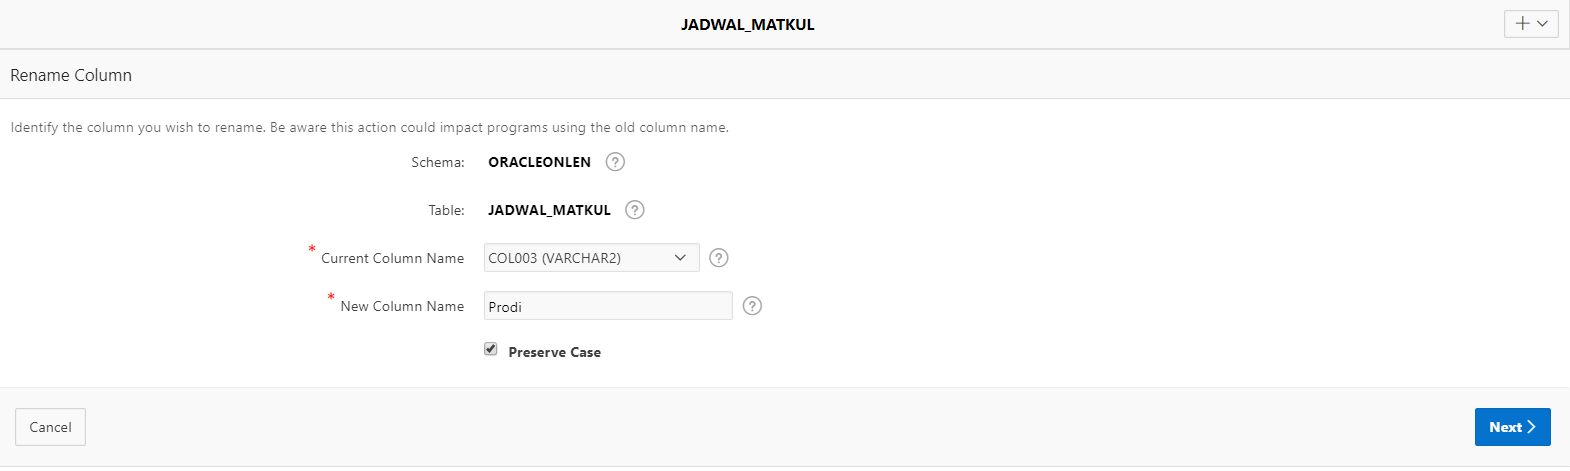
\includegraphics [width=7cm]{figure/Capture11.PNG}
        \caption{Caption}
        \label{fig:my_label}
    \end{figure}
    
    \item Jika sudah dinamai semuanya, maka pilih Creat App
     \begin{figure}[!htbp]
        \centering
        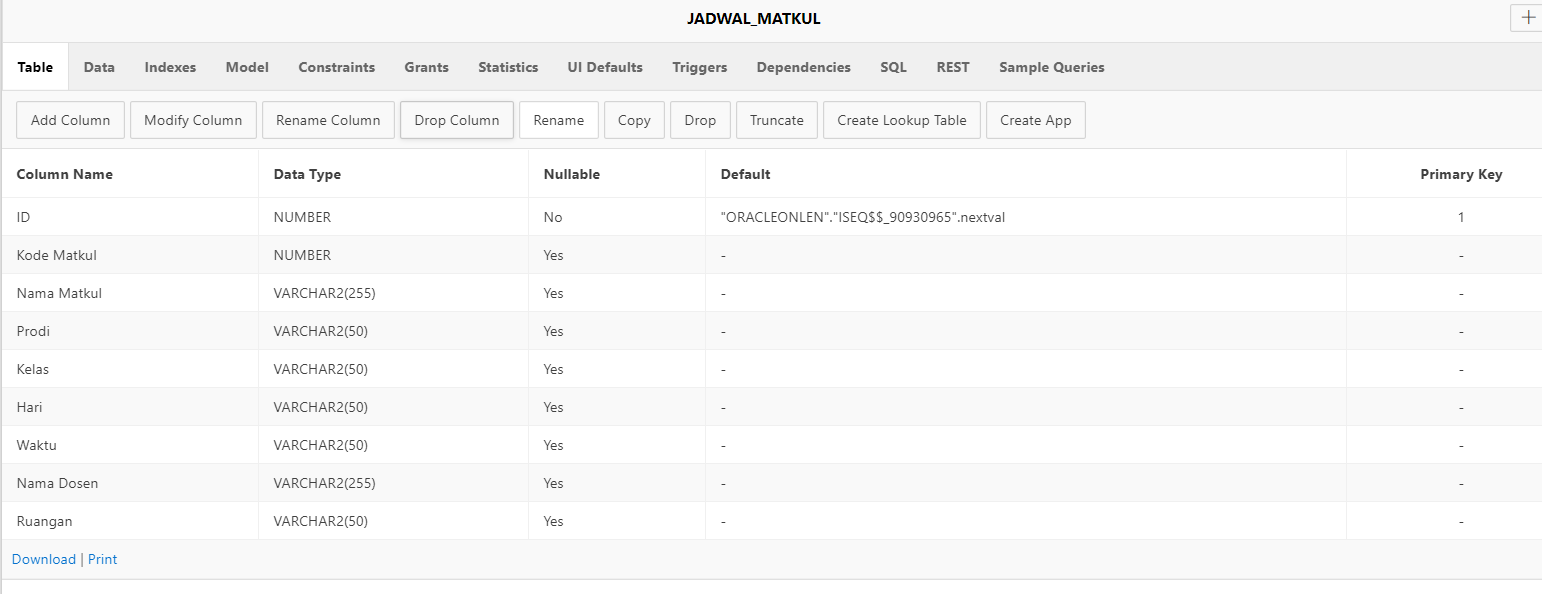
\includegraphics [width=3cm]{figure/Capture12.PNG}
        \caption{Caption}
        \label{fig:my_label}
    \end{figure}
    
    \item Klik Creat Application
    \begin{figure}[!htbp]
        \centering
        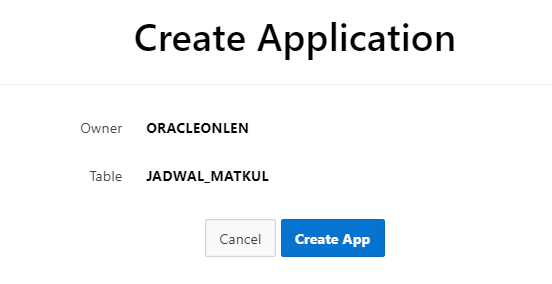
\includegraphics [width=3cm]{figure/Capture13.PNG}
        \caption{Caption}
        \label{fig:my_label}
    \end{figure}
    
    \item Setelah dibuat, jika kalian ingin melihat aplikasi yang kalian buat tadi maka klik Run Application
    \begin{figure}[!htbp]
        \centering
        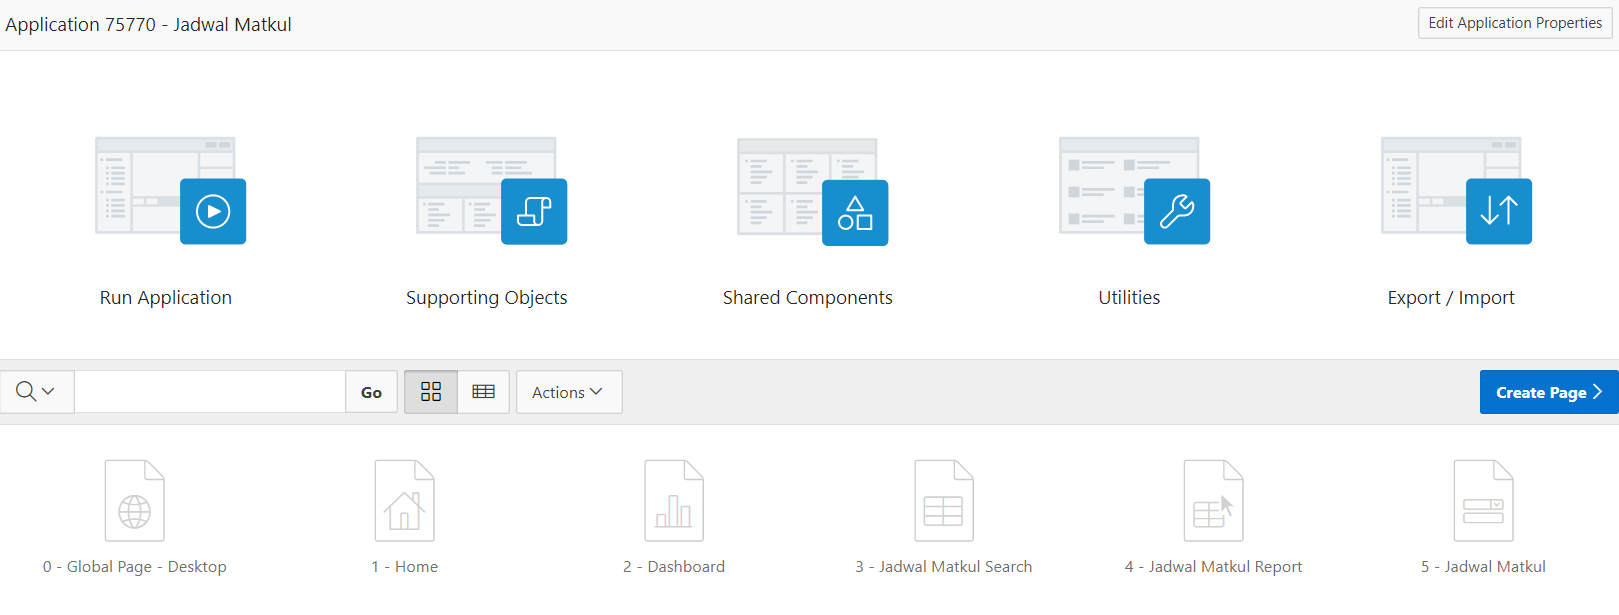
\includegraphics [width=3cm]{figure/Capture7.PNG}
        \caption{Caption}
        \label{fig:my_label}
    \end{figure}
    
    \item Sebelum masuk ke aplikasi yang telah dibuat, kalian harus login dulu terlebih dahulu memakai akun masuk oracle APEX
     \begin{figure}[!htbp]
        \centering
        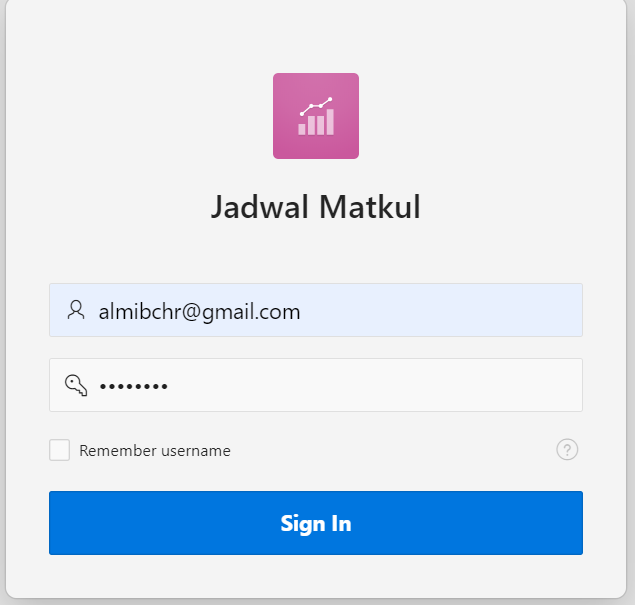
\includegraphics [width=3cm]{figure/Capture8.PNG}
        \caption{Caption}
        \label{fig:my_label}
    \end{figure}
    
    \item Setelah login maka akan masuk ke tampilan awal aplikasi yang telah dibuat
     \begin{figure}[!htbp]
        \centering
        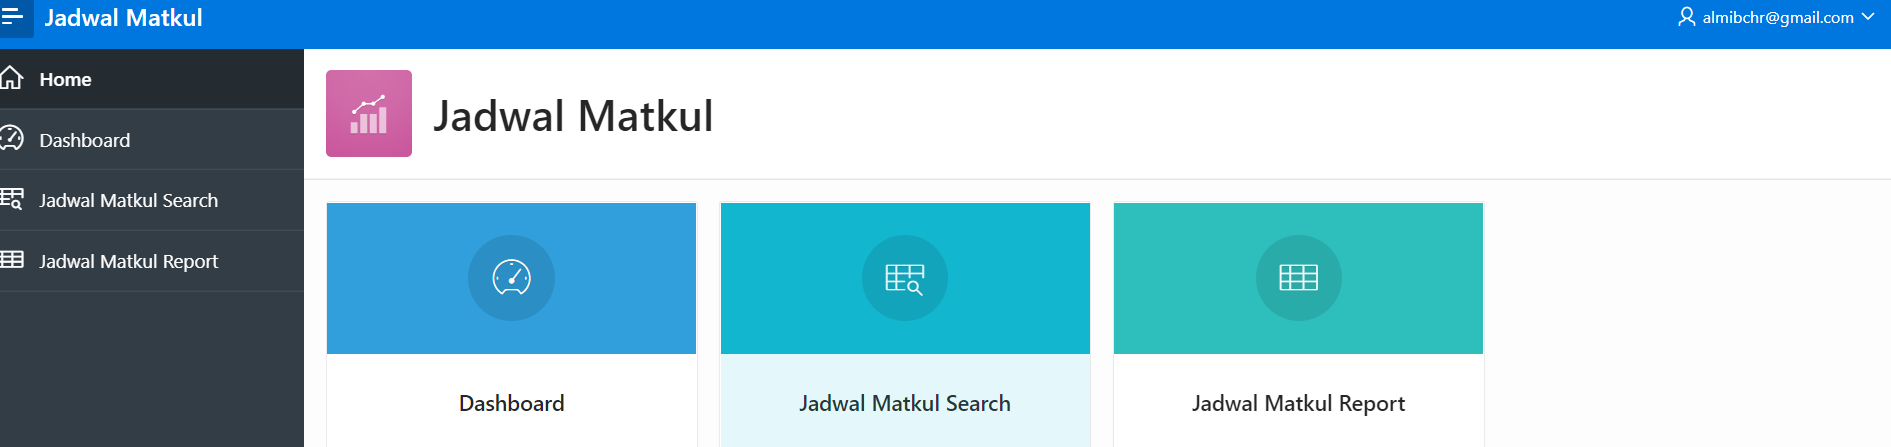
\includegraphics [width=3cm]{figure/Capture9.PNG}
        \caption{Caption}
        \label{fig:my_label}
    \end{figure}
    
    SELESAI !
\end{enumerate}
\end{document}

